\documentclass[11pt]{article}

% --------------------------------------------------
% Packages
% --------------------------------------------------
\usepackage[margin=1in]{geometry}
\usepackage{amsmath, amssymb, amsthm}
\usepackage{mathtools}
\usepackage{graphicx}
\usepackage{float}
\usepackage{enumitem}
\usepackage{hyperref}
\usepackage{xcolor}
\usepackage{tikz}
\usetikzlibrary{arrows.meta, positioning, calc}

% Pseudocode and algorithms
\usepackage{algorithm}
\usepackage{algpseudocode}

% Better fonts (optional)
\usepackage{lmodern}

% --------------------------------------------------
% Hyperref setup
% --------------------------------------------------
\hypersetup{
    colorlinks=true,
    linkcolor=blue,
    citecolor=blue,
    urlcolor=blue
}

% --------------------------------------------------
% Theorem-like environments
% --------------------------------------------------
\theoremstyle{definition}
\newtheorem{definition}{Definition}[section]
\newtheorem{theorem}{Theorem}[section]
\newtheorem{claim}{Claim}[section]
\newtheorem{remark}{Remark}[section]
\newtheorem{recall}{Recall}[section]

\theoremstyle{proof}
% Proof environment is built-in via amsthm

% --------------------------------------------------
% Custom commands
% --------------------------------------------------
\newcommand{\Gen}{\mathsf{Gen}}
\newcommand{\Enc}{\mathsf{Enc}}
\newcommand{\Dec}{\mathsf{Dec}}
\newcommand{\Sig}{\mathsf{Sig}}
\newcommand{\Ver}{\mathsf{Ver}}
\newcommand{\negl}{\mathsf{negl}}

% --------------------------------------------------
% Document
% --------------------------------------------------
\begin{document}

\title{Public Key Crypto notes - 10}
\author{By contributors}
\date{April 20. 2026}
\maketitle

\section{Elliptic curves}

\begin{recall}
	$E_{A, B} = \{(x, y) \in \mathbb{R}^2, y^2 = x^3 + Ax + B\} \cup \{\infty\}, 4A^3 + 27B^2 \ne 0$
\end{recall}

For given $P = (x_P, y_P)$, $Q = (x_Q, y_Q)$, such that $P \ne Q, x_P \ne x_Q$. Let's compute $R = (x_R, y_R), R = P \oplus Q$.

Here, $-R = (x_R, -y_R)$, and $P, Q, -R$ are on $E$, and on the same line.

First, take the line through $P, Q$, $y = m(x-x_P) + y_P$ with slope $m$. Here, the slope $m = \frac{y_Q - y_P}{x_Q - x_P}$. Take the intersection of $E$ with the line.

\begin{align}
	(m (x-x_P) + y_P)^2 &= x^3 + Ax + B \\
	x^3 + m^2x^2 + \dots &= 0 \label{2}\\
	(x-x_P) (x-x_Q) (x-x_R) &= 0 \label{3}\\
	x^3 - (x_P + x_Q + x_R) x^2 + \dots &= 0
\end{align}

So \eqref{2} and \eqref{3} are the same equation and $m^2 = x_P + x_Q + x_R$, i.e. $x_R = m^2 - x_P - x_Q$.

$-R = (x_R - y_R)$ is on the line. So $-y_R = m(x_R - x_P) + y_P$, and $y_R = -m(x_R - x_P) - y_P$.

\begin{theorem}[Group law]
	Let $E: y^2 = x^3 + Ax + B$, $P = (x_P, y_P), Q = (x_Q, y_Q)$. Let $R = P \oplus Q = (x_R, y_R)$. Then:
	
	\begin{enumerate}
		\item If $P, Q \ne \infty, x_P \ne x_Q$:
		\begin{itemize}
			\item $x_R = m^2 - x_P - x_Q, m = \frac{y_Q - y_P}{x_Q - x_P}$
			\item $y_R = -m (x_R - x_P) - y_P$
		\end{itemize}
		\item If $P = Q$, but $y_P \ne 0$:
		\begin{itemize}
			\item $x_R = m^2 - 2x_P, m = \frac{3x_P^2 + A}{2y_P}$
			\item $y_R = -m(x_R - x_P) - y_P$
		\end{itemize}
		\item If $x_P = x_Q$:
		\begin{itemize}
			\item $R = \infty$
		\end{itemize}
		\item If $P = Q, y_P = 0$:
		\begin{itemize}
			\item $R = \infty$
		\end{itemize}
		\item $\infty + P = P + \infty = P$
	\end{enumerate}
	
	Then, the curve $E$ with $\oplus$ forms a group, i.e.:
	
	\begin{itemize}
		\item If $P, Q \in E \rightarrow P \oplus Q \in E$
		\item $\infty$ serves as the null element, such that $\infty \oplus P = P \oplus \infty = P$
		\item There is a negation, i.e. for all $P$, there is a $Q$, such that $P \oplus Q = \infty$ (This is true when $P = (x_P, y_P) \rightarrow Q = (x_P, -y_P)$)
		\item $\oplus$ is commutative, i.e. $P \oplus Q = Q \oplus P$
		\item $\oplus$ is associative, i.e. $P \oplus (Q \oplus R) = (P \oplus Q) \oplus R$
	\end{itemize}
\end{theorem}

\begin{proof}
	We will not prove this theorem.
\end{proof}

\section{Elliptic curves modulo $P$}

\begin{definition}
	Let $p > 3$ be a prime and $E_{A, B} = \{y^2 = x^3 + Ax + B \pmod{p}\} \cup \infty$ with $4A^3 + 27B^2 \ne 0 \pmod{p}$
\end{definition}

\begin{remark}
	Everything works as before, but with modular arithmetic modulo $p$.
\end{remark}

Example: $E: y^2 = x^3 + x + 1 \pmod{5}$

We first check whether this is a valid elliptic curve: $4A^3 + 27B^2 = 4 + 27 = 31 \not \equiv 0 \mod{5}$

\vspace{1em}
\begin{center}
	\begin{tabular}{|c|c|c|c|}
		\hline
		$x$ & $x^3 + x + 1$ & $y$ & points \\ \hline
		0 & 1 & $\pm 1$ & $(0, 1), (0, 4)$ \\ \hline
		1 & 3 & - & - \\ \hline
		2 & 1 & $\pm 1$ & $(2, 1), (2, 4)$ \\ \hline
		3 & 1 & $\pm 1$ & $(3, 1), (3, 4)$ \\ \hline
		4 & 4 & $\pm 2$ & $(4, 2), (4, 3)$ \\ \hline
		\multicolumn{4}{|c|}{$\infty$} \\ \hline
	\end{tabular}	
\end{center}
\vspace{1em}

$|E| = 9$

\begin{figure}
	\centering
	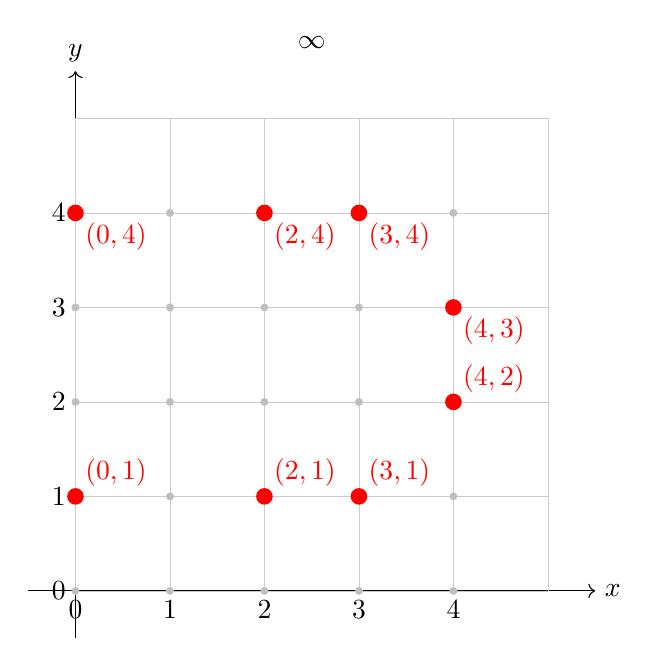
\begin{tikzpicture}[scale=1.2]
		
		% Axes
		\draw[->] (-0.5,0) -- (5.5,0) node[right] {$x$};
		\draw[->] (0,-0.5) -- (0,5.5) node[above] {$y$};
		
		% Grid
		\draw[step=1, gray!40, very thin] (0,0) grid (5,5);
		
		% Tick labels
		\foreach \x in {0,1,2,3,4}
		\node[below] at (\x,0) {\x};
		\foreach \y in {0,1,2,3,4}
		\node[left] at (0,\y) {\y};
		
		% All lattice points (optional faint background points)
		\foreach \x in {0,1,2,3,4}{
			\foreach \y in {0,1,2,3,4}{
				\fill[gray!50] (\x,\y) circle (1.2pt);
			}
		}
		
		% Highlight elliptic curve points
		\foreach \P/\label in {
			0/1/{(0,1)},
			0/4/{(0,4)},
			2/1/{(2,1)},
			2/4/{(2,4)},
			3/1/{(3,1)},
			3/4/{(3,4)},
			4/2/{(4,2)},
			4/3/{(4,3)}
		}{
			\fill[red] (\P,\label) circle (2.5pt);
		}
		
		% Labels for highlighted points
		\node[above right, red] at (0,1) {$(0,1)$};
		\node[below right, red] at (0,4) {$(0,4)$};
		\node[above right, red] at (2,1) {$(2,1)$};
		\node[below right, red] at (2,4) {$(2,4)$};
		\node[above right, red] at (3,1) {$(3,1)$};
		\node[below right, red] at (3,4) {$(3,4)$};
		\node[above right, red] at (4,2) {$(4,2)$};
		\node[below right, red] at (4,3) {$(4,3)$};
		
		% Point at infinity note
		\node at (2.5,5.8) {$\infty$};
		
	\end{tikzpicture}
	\caption{The points of \(E: y^2 \equiv x^3 + x + 1 \pmod{5}\) in \(\mathbb{F}_5^2\), with the point at infinity \(\infty\).}
\end{figure}

Let's compute $(3, 1) \oplus (2, 4)$:

\begin{align}
	m = \frac{1-4}{3-2} &= -3 = 2 \\
	x_R = m^2 - 3 - 2 &= 4 - 3 - 2 = 4 \\
	y_R = -m (4-3) - 1 &= -2 \cdot 1 -1 = -3 = 2 \rightarrow \\
	\rightarrow (x_R, y_R) &= (4, 2)
\end{align}

\begin{remark}
	$E = \{n \cdot (0, 1) \cdot n = 0, \dots, 8\}$, where $(0, 1) \oplus (0, 1) \oplus \dots \oplus (0, 1) = nx$.
	
	$p \cdot (0, 1) = \infty = 0 \cdot (0, 1) \rightarrow E \stackrel{\sim}{=} \mathbb{Z}_9$
\end{remark}

\begin{theorem}[Hasse-Weil]
	Let $E$ be an elliptic curve modulo $p$. Then: $||E| = (p + 1)| \le 2\sqrt{p}$.
\end{theorem}

\begin{theorem}
	Let $E$ be an elliptic curve modulo $p$. Then, $E \stackrel{\sim}{=} \mathbb{Z}_N$ or $E = \mathbb{Z}_N \times \mathbb{Z}_M$ with $M | N$.
	
	That is, either:
	
	\begin{itemize}
		\item $E = \{n \cdot P, n \in \mathbb{Z}_N\}$ for some $P \in E$ (special case: $|E| = N$), or
		\item $E = \{n \cdot P + kQ, n \in \mathbb{Z}_N, k \in \mathbb{Z}_M\}$ for some $P, Q \in E$. This is unique (special case: $|E| = N \cdot M$)
	\end{itemize}
\end{theorem}

\end{document}